\documentclass[12pt,a4paper]{article}
\usepackage[utf8]{inputenc}
\usepackage[T1]{fontenc}
\usepackage{amsmath}
\usepackage{amsfonts}
\usepackage{amssymb}
\usepackage{graphicx}
\usepackage[indonesian]{babel}
\usepackage[left=2.00cm, right=2.00cm, top=2.00cm, bottom=2.00cm]{geometry}
\usepackage{float} 

\title{Tugas 13 - Pengolahan Sinyal Digital\\
	Struktur Jaringan untuk Sistem Finite Impulse Response (FIR)}

% remove spacing around date:
\usepackage{titling}
\predate{}
\postdate{}
\date{}

\begin{document}
	\maketitle
	\date{}
	\begin{enumerate}
		\item Diketahui $ H(z) $ yang merepresentasikan system function untuk sistem sebagai berikut:
		\[ H(z) = \left( 1 + \frac{1}{2}z^{-1} \right) \left( 1 + 2z^{-1} \right) \left( 1 - \frac{1}{4}z^{-1} \right) \left( 1 - 4z^{-1} \right)\]
		Gambarlah grafik aliran sinyalnya untuk mengimplementasikan sistem ini dalam bentuk-bentuk berikut ini:
		\begin{enumerate}
			\item cascade form\\
			\textbf{Jawaban:} Karena hanya memiliki real zeros maka hanya gunakan orde pertama dalam cascade form-nya
			\begin{figure}[H]
				\centering
				
\includegraphics[width=0.7\linewidth]{img/img01}
			\end{figure}
			\item direct form
			\textbf{Jawaban:} Kita ekspresikan H(z) sebagai 
			\begin{figure}[H]
				\centering
				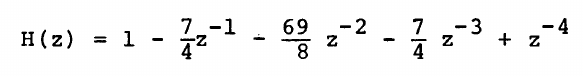
\includegraphics[width=0.5\linewidth]{img/img02}
			\end{figure}
			kemudian struktur direct-form-nya adalah
			\begin{figure}[H]
				\centering
				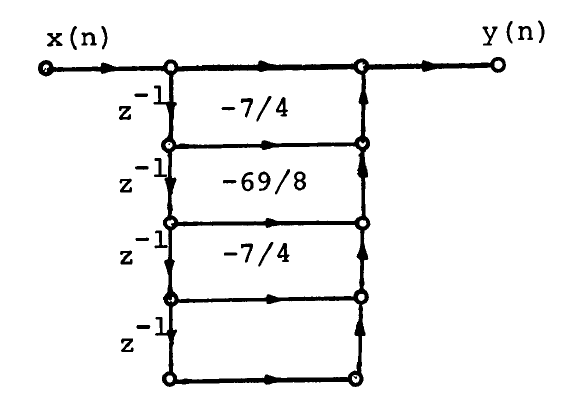
\includegraphics[width=0.5\linewidth]{img/img03}
			\end{figure}
			\item linear-phase form\\
			\textbf{Jawaban:}
			\begin{figure}[H]
				\centering
				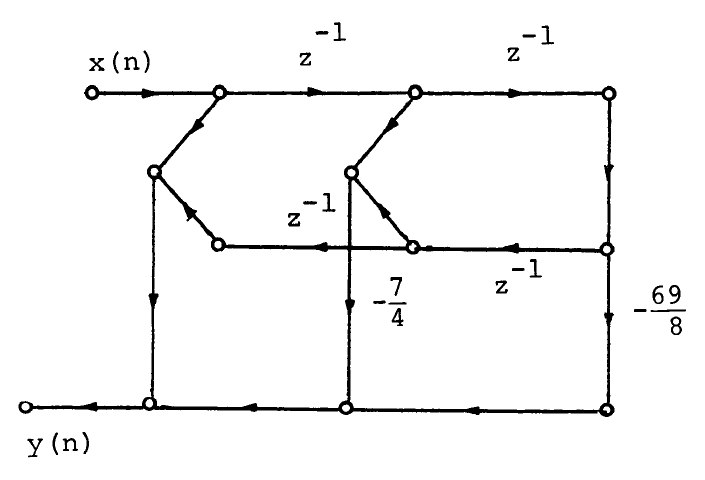
\includegraphics[width=0.5\linewidth]{img/img04}
			\end{figure}
		\end{enumerate}
	\end{enumerate}
\end{document}